\documentclass[11pt,a4paper]{article}

\usepackage[provide=*,spanish]{babel}
\usepackage[utf8]{inputenc}
\usepackage[T1]{fontenc}
\usepackage{lmodern}
\usepackage[margin=2.35cm]{geometry}
\usepackage{amsmath}
\usepackage{booktabs}
\usepackage{longtable}
\usepackage{tabularx}
\usepackage{array}
\usepackage{enumitem}
\usepackage{listings}
\usepackage{xcolor}
\usepackage{microtype}
\usepackage{parskip}
\usepackage{titlesec}
\usepackage{hyperref}
\usepackage{graphicx}
\usepackage{caption}
\usepackage{subcaption}
\usepackage{float}

\definecolor{azulWCD}{RGB}{17,67,112}
\definecolor{azulClaro}{RGB}{232,241,249}
\definecolor{grisCodigo}{RGB}{247,247,247}
\definecolor{verdeCodigo}{RGB}{25,110,55}
\definecolor{rojoCodigo}{RGB}{145,35,35}
\definecolor{tituloColor}{RGB}{0,55,110}
\definecolor{reglaColor}{RGB}{0,90,160}

\hypersetup{
  colorlinks=true,
  linkcolor=azulWCD,
  urlcolor=azulWCD,
  citecolor=azulWCD,
  pdftitle={Caracterizacion del proceso de moderacion y captura de neutrones termicos en el WCD},
  pdfauthor={Jaime A. Betancourt}
}

\lstdefinestyle{pystyle}{
  language=Python,
  backgroundcolor=\color{grisCodigo},
  basicstyle=\ttfamily\footnotesize,
  keywordstyle=\color{azulWCD}\bfseries,
  commentstyle=\color{verdeCodigo}\itshape,
  stringstyle=\color{rojoCodigo},
  breaklines=true,
  breakatwhitespace=false,
  frame=single,
  rulecolor=\color{gray!40},
  tabsize=2,
  showstringspaces=false,
  columns=fullflexible,
  keepspaces=true
}
\lstset{style=pystyle}

\titleformat{\section}{\normalfont\Large\bfseries\color{azulWCD}}
  {\thesection.}{0.6em}{}
\titleformat{\subsection}{\normalfont\large\bfseries}
  {\thesubsection.}{0.5em}{}
\setlist{itemsep=0.25em,topsep=0.4em}
\renewcommand{\arraystretch}{1.18}
\setlength{\emergencystretch}{2em}

\newcommand{\codigo}[1]{\nolinkurl{#1}}
\newcommand{\archivo}[1]{\path{#1}}
\newcommand{\var}[1]{\texttt{#1}}

\begin{document}
\pagestyle{empty}

%------------------------------------------------
% PORTADA
%------------------------------------------------

\begin{titlepage}
\begin{center}

\vspace*{0.5cm}
\textcolor{reglaColor}{\rule{\linewidth}{1.2pt}}

\vspace{1.3cm}
{\Large\scshape Universidad Industrial de Santander}\\[0.2cm]
{\large Escuela de Física --- Facultad de Ciencias}\\[0.2cm]
{\large Doctorado en Física}

\vspace{2.2cm}
{\Huge\bfseries\color{tituloColor} Caracterización del proceso de\\[0.2cm]
moderación y captura de neutrones\\[0.2cm] térmicos en el WCD}

\vspace{1.8cm}
{\large\textbf{Informe técnico}}

\vspace{0.6cm}
\begin{minipage}{0.82\linewidth}
\centering
\textit{``Variables de análisis para su futuro uso como instrumento de medición de humedad y
salinidad del suelo''}
\end{minipage}

\vfill

{\large\textbf{Autor}}\\[0.15cm]
Jaime A. Betancourt\\[0.1cm]
Doctorado en Física, Universidad Industrial de Santander

\vspace{1.2cm}
\textcolor{reglaColor}{\rule{0.5\linewidth}{0.6pt}}

\vspace{1cm}
15 de septiembre de 2026

\vspace{1cm}
\textcolor{reglaColor}{\rule{\linewidth}{1.2pt}}

\end{center}
\end{titlepage}

\pagestyle{plain}

\begin{abstract}
Este informe documenta e interpreta, para un lector con acceso al repositorio de la tesis pero sin
conocimiento previo del análisis, el conjunto de variables físicas que se calculan a partir de las
simulaciones Monte Carlo (Geant4/MEIGA) del detector Cherenkov de agua (WCD) con agua pura y con
soluciones de NaCl, mediante el \textit{notebook} \codigo{analisis\_moderacion\_captura\_neutrones.ipynb}.
Se explica el significado físico y el propósito de cada variable --coeficiente de captura en el
medio, reflexión, transmisión, número de dispersiones elásticas $N$, letargía logarítmica $\xi$,
tiempo hasta la captura $\Delta t$ y su tiempo de decaimiento (\textit{die-away}) $\tau$, e
interacciones previas con el acero inoxidable, el Tyvek y el aire-- y se justifica por qué esta
caracterización es un paso necesario antes de poder emplear el WCD como un instrumento de campo
para estimar humedad del suelo mediante la técnica de sensado cósmico de neutrones
(CRNS). Se presentan resultados comparativos entre agua pura y agua con 2.5\,\% de NaCl como
ejemplo ilustrativo del método.
\end{abstract}

\tableofcontents

\section{Objeto y alcance del informe}

El detector Cherenkov de agua (\textit{Water Cherenkov Detector}, WCD) que se modela en esta tesis
responde, en última instancia, a neutrones que se moderan y se capturan dentro de su volumen
sensible. Antes de poder interpretar la señal que un WCD real produciría en campo y de poder
relacionar esa señal con la humedad del suelo bajo el detector es necesario
caracterizar, mediante simulación controlada, \emph{cómo} un neutrón que ingresa al tanque se
comporta: cuántos de ellos son efectivamente capturados dentro del medio activo, cuántos rebotan
sin llegar a ingresar, cuántos atraviesan el tanque sin ser capturados, cuánto tardan en capturarse
y cuántas colisiones elásticas experimentan en el camino.

Este informe documenta el análisis que resuelve esa caracterización a partir de una corrida de
100\,000 neutrones primarios inyectados a 25\,meV (neutrones ya termalizados), y explica el
significado de cada variable calculada para un lector que solo tiene acceso al repositorio de la
tesis y a los archivos de salida, no a esta conversación. El análisis en sí --el código, los
archivos de entrada y las figuras-- vive en el \textit{notebook}
\codigo{analisis\_moderacion\_captura\_neutrones.ipynb}, que se ejecuta de forma independiente para
cada medio (agua pura, agua con distintas concentraciones de NaCl); ver la sección~\ref{sec:reprod}
para su ubicación y forma de reproducirlo.

\section{Contexto: por qué se caracteriza así un detector de humedad de suelo}
\label{sec:contexto}

La técnica de \textbf{sensado cósmico de neutrones} (\textit{Cosmic-Ray Neutron Sensing}, CRNS) mide
la humedad del suelo de forma no invasiva a partir de un hecho físico simple: el hidrógeno es, por
mucho, el núcleo más eficiente para moderar (frenar) neutrones rápidos producidos por la radiación
cósmica en la atmósfera. Cuanta más agua contiene el suelo bajo un detector, más se moderan y se
absorben los neutrones que provienen del suelo, y por tanto \emph{menor} es el flujo de neutrones
epitérmicos/rápidos que un detector situado sobre la superficie llega a contar. Un WCD --diseñado
originalmente para detectar muones y electrones mediante luz Cherenkov-- puede, en principio,
adaptarse para actuar como uno de estos detectores de neutrones si su respuesta a la captura de
neutrones térmicos dentro de su propio tanque de agua está bien caracterizada.

Esa caracterización es exactamente lo que documenta este informe. Las variables que se describen en
la sección~\ref{sec:variables} no son un ejercicio académico aislado: cada una tiene una lectura
directa en términos de la futura aplicación del WCD como instrumento de campo:

\begin{itemize}
  \item El \textbf{coeficiente de captura en el medio} cuantifica qué fracción de los neutrones que
  llegan al detector realmente producen una señal utilizable (captura seguida de emisión gamma y,
  eventualmente, luz Cherenkov). Es, en esencia, la \emph{eficiencia intrínseca} del WCD como
  detector de neutrones.
  \item La \textbf{reflexión} y la \textbf{transmisión} cuantifican, respectivamente, qué fracción
  de neutrones nunca llega a ``verse'' por el detector y qué fracción lo atraviesa sin dejar señal
  --dos formas distintas de pérdida de sensibilidad que conviene distinguir al diseñar la geometría
  del tanque (altura, blindaje, posición del PMT).
  \item El \textbf{número de dispersiones elásticas} $N$ y la \textbf{letargía} $\xi$ describen el
  camino de termalización del neutrón dentro del agua: son las variables clásicas con las que la
  física de reactores caracteriza el poder moderador de un medio, y aquí sirven para verificar que
  el tratamiento térmico de la simulación (ligado por hidrógeno, ver la nota de S($\alpha,\beta$) en
  la sección~\ref{sec:sim}) se comporta como se espera físicamente.
  \item El \textbf{tiempo hasta la captura} $\Delta t$ y, en particular, el \textbf{tiempo de
  decaimiento} $\tau$ ajustado a su distribución son la variable con la conexión más directa a la
  instrumentación real: en la industria de pozos petroleros, la técnica de registro de neutrones
  pulsados (\textit{pulsed neutron logging}) mide exactamente esta misma curva de decaimiento
  (\textit{die-away}) de la población térmica de neutrones para inferir la porosidad y, sobre todo,
  la \textbf{salinidad} del fluido que rodea la sonda --porque el cloro es un absorbente de
  neutrones térmicos mucho más fuerte que el hidrógeno o el oxígeno. Esta tesis reproduce esa misma
  física dentro de un WCD: $\tau$ (o, de forma equivalente, el coeficiente de captura) es
  potencialmente el observable que permitiría, con la calibración adecuada, separar el efecto de la
  \emph{humedad} (cuánta agua hay) del efecto de la \emph{salinidad} (cuánta sal hay disuelta en esa
  agua) en una medición real de campo.
  \item Las \textbf{interacciones con el acero inoxidable, el Tyvek y el aire} antes de que el
  neutrón ingrese al medio activo caracterizan cuánto ``distorsiona'' la estructura mecánica del
  tanque la señal que en principio debería depender solo de la humedad/salinidad del suelo --
  información relevante para el diseño de futuras versiones del detector.
\end{itemize}

En resumen: este análisis traduce una simulación de transporte de neutrones a un conjunto pequeño
de números y curvas que se pueden comparar directamente contra la teoría de moderación/difusión de
neutrones y, más adelante, contra mediciones de campo -- ese es el puente entre "simular el WCD" y
"usar el WCD para medir humedad de suelo".

\section{Configuración de la simulación}
\label{sec:sim}

Cada corrida analizada en este informe simula \textbf{100\,000 neutrones primarios}, inyectados
verticalmente hacia abajo desde \textbf{2\,m} de altura sobre el tanque, con una energía inicial
monoenergética de \textbf{25\,meV} (es decir, neutrones que parten ya termalizados, para aislar el
comportamiento del detector del proceso de termalización atmosférica). El tanque es cilíndrico, de
\textbf{1.33\,m} de altura, con cuerpo de \textbf{acero inoxidable} y revestimiento interno de
\textbf{Tyvek}; el fotomultiplicador (PMT) está bajo la tapa interna, a \textbf{$\sim$26\,cm} de
profundidad. El medio activo del tanque es agua pura o una solución de NaCl a una concentración
dada (2.5\,\%, 5\,\%, 10\,\% en masa, según la corrida).

El transporte de neutrones usa Geant4 con física de alta precisión (\codigo{QGSP\_BERT\_HP}) y, de
forma crucial para la física de baja energía que aquí interesa, el tratamiento térmico
$S(\alpha,\beta)$ para el hidrógeno ligado en moléculas de agua (\codigo{G4ThermalNeutrons}), que
permite representar correctamente la dispersión elástica \emph{y} el \textit{up-scattering} térmico
(ganancia de energía en una colisión) cerca del equilibrio térmico -- un efecto que la física de
neutrones libres/gas ideal no captura y que resulta visible en los resultados de la
sección~\ref{sec:xi}.

\section{Trazabilidad de los datos: de la simulación a las variables}
\label{sec:pipeline}

Geant4 registra, paso a paso, el transporte de cada neutrón en cuatro archivos TSV que el
\textit{notebook} combina mediante un identificador común, \var{run\_id} (un entero de 0 a 99\,999,
uno por cada neutrón primario inyectado):

\begin{itemize}
  \item \archivo{neutrones-incidentes.tsv}: un registro por cada uno de los 100\,000 neutrones
  inyectados (su paso inicial, siempre en aire). Es el universo de referencia contra el que se
  calculan todos los porcentajes de este informe.
  \item \archivo{pasos-neutrones.tsv}: el historial \emph{completo} de cada neutrón, paso a paso,
  incluyendo los pasos de puro transporte (cruces de frontera entre materiales).
  \item \archivo{interacciones-neutrones.tsv}: el mismo historial, pero sin los pasos de puro
  transporte -- solo dispersiones elásticas (\var{hadElastic}), capturas (\var{nCapture}) y, en
  menor medida, interacciones inelásticas.
  \item \archivo{capturas-neutrones.tsv}: únicamente las filas donde ocurrió una captura
  (\var{nCapture}), en cualquier material, con el núcleo capturador identificado
  (\var{target\_Z}/\var{target\_A}).
\end{itemize}

A partir de estos cuatro archivos, el \textit{notebook} construye, en orden: (1) el subconjunto de
capturas que ocurrieron específicamente dentro del medio activo; (2) su verificación contra el
registro de inyección; (3) el tramo de la trayectoria de cada neutrón capturado que va desde su
\emph{primera} dispersión elástica hasta su captura (el ``ciclo de moderación''); y (4) el mismo
tramo tomado de \archivo{interacciones-neutrones.tsv}, usado como fuente de verificación cruzada
independiente. Todas las variables descritas en la sección~\ref{sec:variables} se derivan de estos
subconjuntos ya verificados.

\section{Variables analizadas}
\label{sec:variables}

\subsection{Medio detector: qué cuenta como ``captura útil''}

No toda captura de un neutrón dentro del tanque es una captura ``en el medio detector''. Un neutrón
puede capturarse en el acero de la carcasa, en el Tyvek del revestimiento o incluso en el nitrógeno
del aire remanente -- estas capturas no producen la señal de interés y se excluyen explícitamente.
El medio detector se identifica por el nombre del material (contiene la palabra \var{Water} en los
archivos de esta simulación, sea agua pura o agua con NaCl) \emph{y} por el núcleo capturador
esperado en ese medio: hidrógeno y oxígeno para agua pura; adicionalmente sodio y cloro cuando hay
NaCl en solución. Esta lista de núcleos válidos (\var{NUCLEOS\_MEDIO\_DETECTOR} en el código) es el
único parámetro que cambia entre corridas de distinta concentración.

\subsection{Coeficiente de captura, reflexión y transmisión}
\label{sec:balance}

Los 100\,000 neutrones inyectados se clasifican en cuatro categorías mutuamente excluyentes:

\begin{itemize}
  \item \textbf{Capturado en el medio}: el neutrón fue absorbido dentro del volumen activo, sobre
  uno de los núcleos válidos de esa corrida. Es la señal ``útil'' del detector.
  \item \textbf{Capturado en otro material}: absorbido en la estructura (acero, Tyvek) o en el aire
  remanente -- señal perdida.
  \item \textbf{Transmitido}: el neutrón llegó a ingresar al medio activo (se detectó al menos una
  interacción suya dentro de él) pero lo abandonó sin ser capturado.
  \item \textbf{Reflejado}: el neutrón nunca llegó a ingresar al medio activo; fue devuelto hacia la
  región de incidencia por la estructura del tanque (o por el propio aire) antes de alcanzar el agua.
\end{itemize}

Estas cuatro fracciones suman 100\,\% de los neutrones inyectados y ofrecen una primera fotografía
del balance global del detector. La figura~\ref{fig:balance} muestra este balance para agua pura.

\begin{figure}[H]
  \centering
  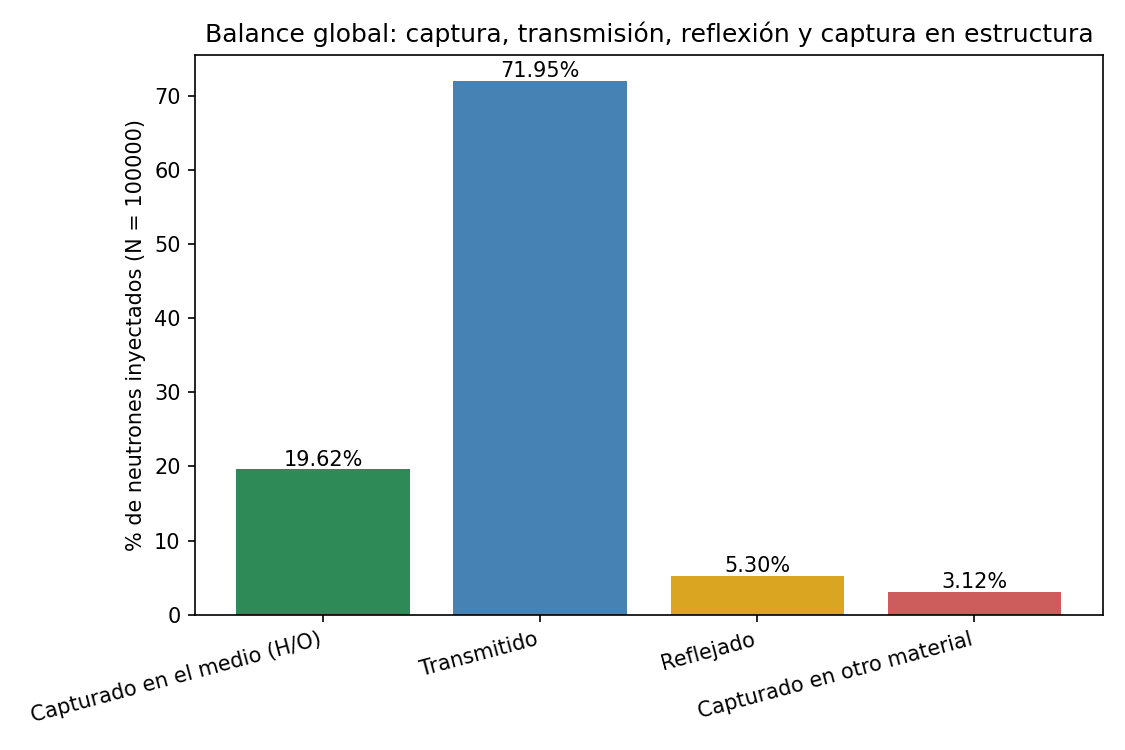
\includegraphics[width=0.72\linewidth]{figuras-analisis-moderacion/agua-pura_05_balance.png}
  \caption{Balance global de los 100\,000 neutrones inyectados (agua pura, 25\,meV): captura en el
  medio, transmisión, reflexión y captura en la estructura.}
  \label{fig:balance}
\end{figure}

\subsection{Número de dispersiones elásticas antes de la captura, $N$}

Cada colisión elástica (\var{hadElastic}) que un neutrón sufre en el agua antes de capturarse es un
evento de moderación: el neutrón intercambia energía con un núcleo del medio y cambia de dirección.
$N$ es, por neutrón capturado en el medio, el número total de esas colisiones. Su distribución
normalizada $P(N\mid\text{captura, medio})$ describe qué tan ``larga'' es, en promedio, la
trayectoria de termalización de un neutrón dentro del detector antes de ser absorbido -- una medida
directa de la difusividad/poder moderador efectivo del medio. La figura~\ref{fig:N} muestra esta
distribución para agua pura, con el pico ajustado por una parábola, el ancho a media altura (FWHM) y
una tabla resumen (mismo formato que las figuras comparativas por energía usadas en el resto de la
tesis).

\begin{figure}[H]
  \centering
  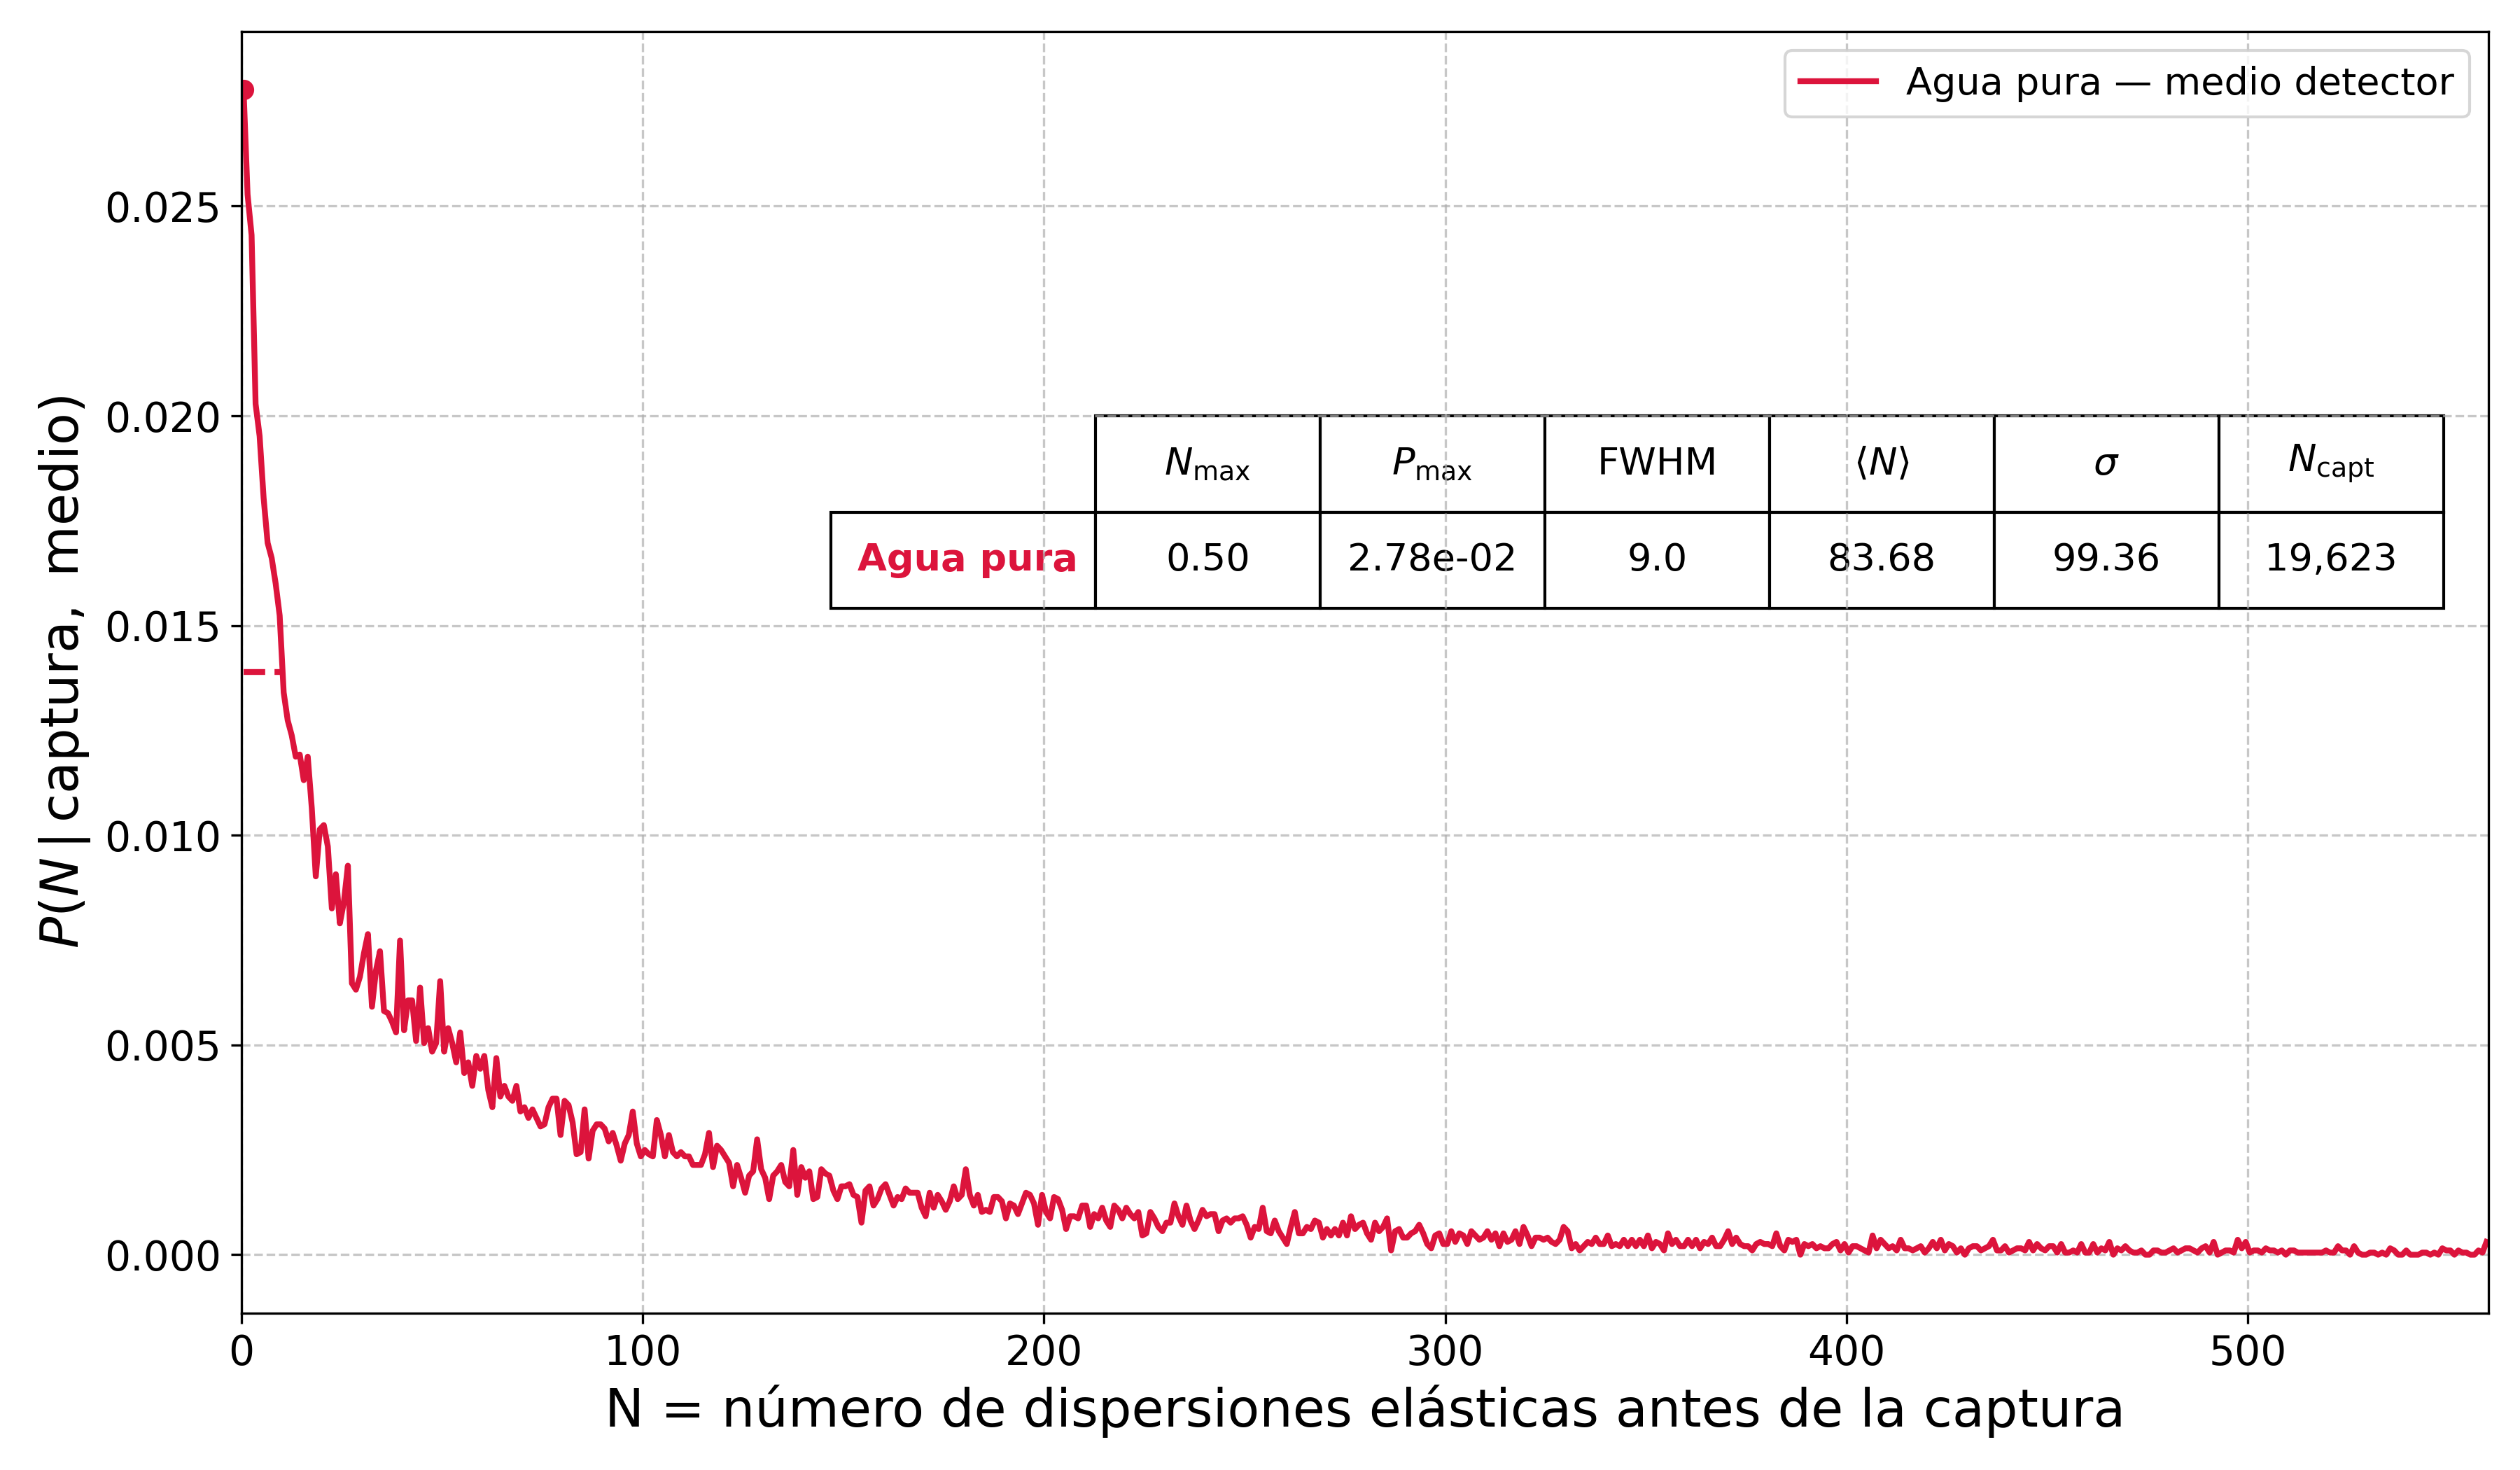
\includegraphics[width=\linewidth]{figuras-analisis-moderacion/agua-pura_06b_N.png}
  \caption{Distribución normalizada de $N$ (agua pura): la mayoría de los neutrones se capturan tras
  relativamente pocas colisiones, pero existe una cola larga hasta $N\approx1600$.}
  \label{fig:N}
\end{figure}

\subsection{Letargía logarítmica, $\xi$}
\label{sec:xi}

La letargía logarítmica es la variable estándar de la física de reactores para cuantificar cuánta
energía pierde (o gana) un neutrón, en promedio, por colisión elástica:
\begin{equation}
  \xi = \ln\!\left(\frac{E_{\text{pre}}}{E_{\text{post}}}\right),
\end{equation}
evaluada en cada colisión \var{hadElastic}. En el régimen clásico de frenado de neutrones rápidos,
$\xi$ es positivo y constante (para hidrógeno libre, $\xi_H\approx1$). Aquí, sin embargo, los
neutrones ya llegan termalizados (25\,meV) y colisionan con hidrógeno \emph{ligado} en moléculas de
agua, tratado con el modelo $S(\alpha,\beta)$: cerca del equilibrio térmico las colisiones pueden
ganar energía tanto como perderla, y el valor medio de $\xi$ se acerca a cero (ligeramente negativo
en los resultados obtenidos). Este resultado no es un error: es la confirmación de que el modelo
térmico de la simulación reproduce el comportamiento físico esperado para neutrones ya
termalizados, y sirve como verificación cruzada de la física del modelo antes de confiar en el
resto de los resultados. La figura~\ref{fig:xi} compara la curva de $\xi$ para agua pura y para
agua con 2.5\,\% de NaCl.

\begin{figure}[H]
  \centering
  \begin{subfigure}[b]{0.49\linewidth}
    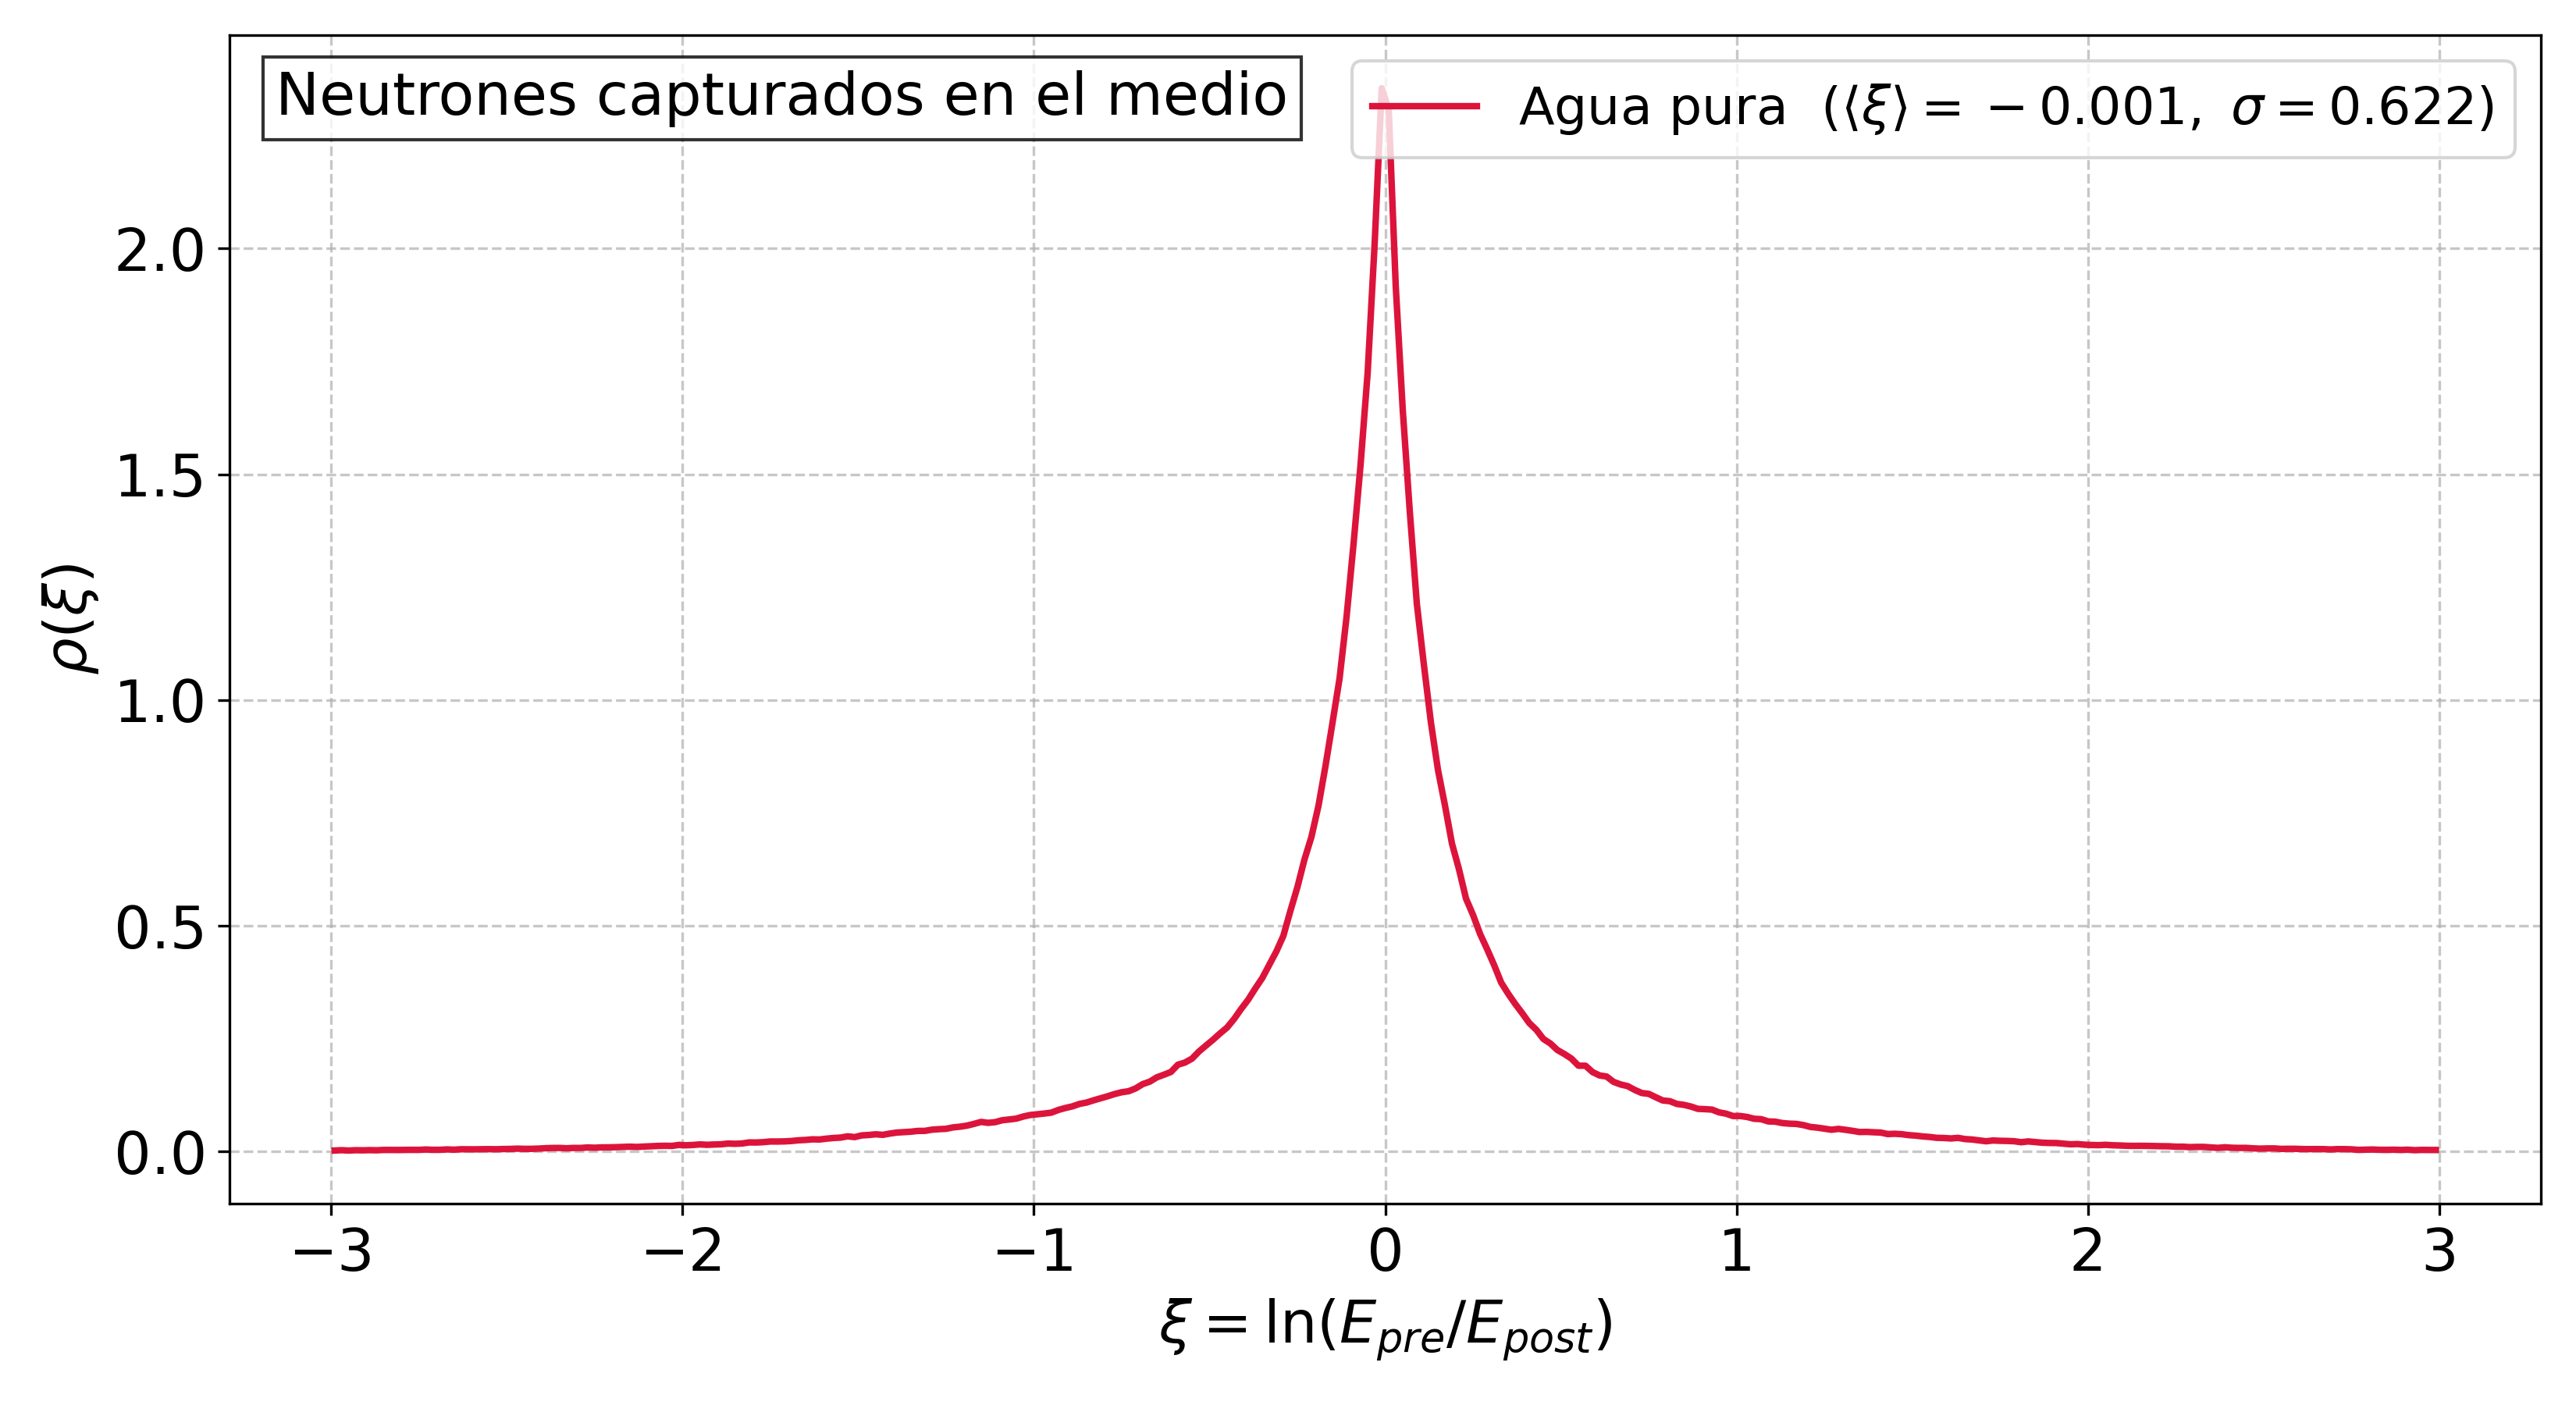
\includegraphics[width=\linewidth]{figuras-analisis-moderacion/agua-pura_06a_xi.png}
    \caption{Agua pura}
  \end{subfigure}
  \hfill
  \begin{subfigure}[b]{0.49\linewidth}
    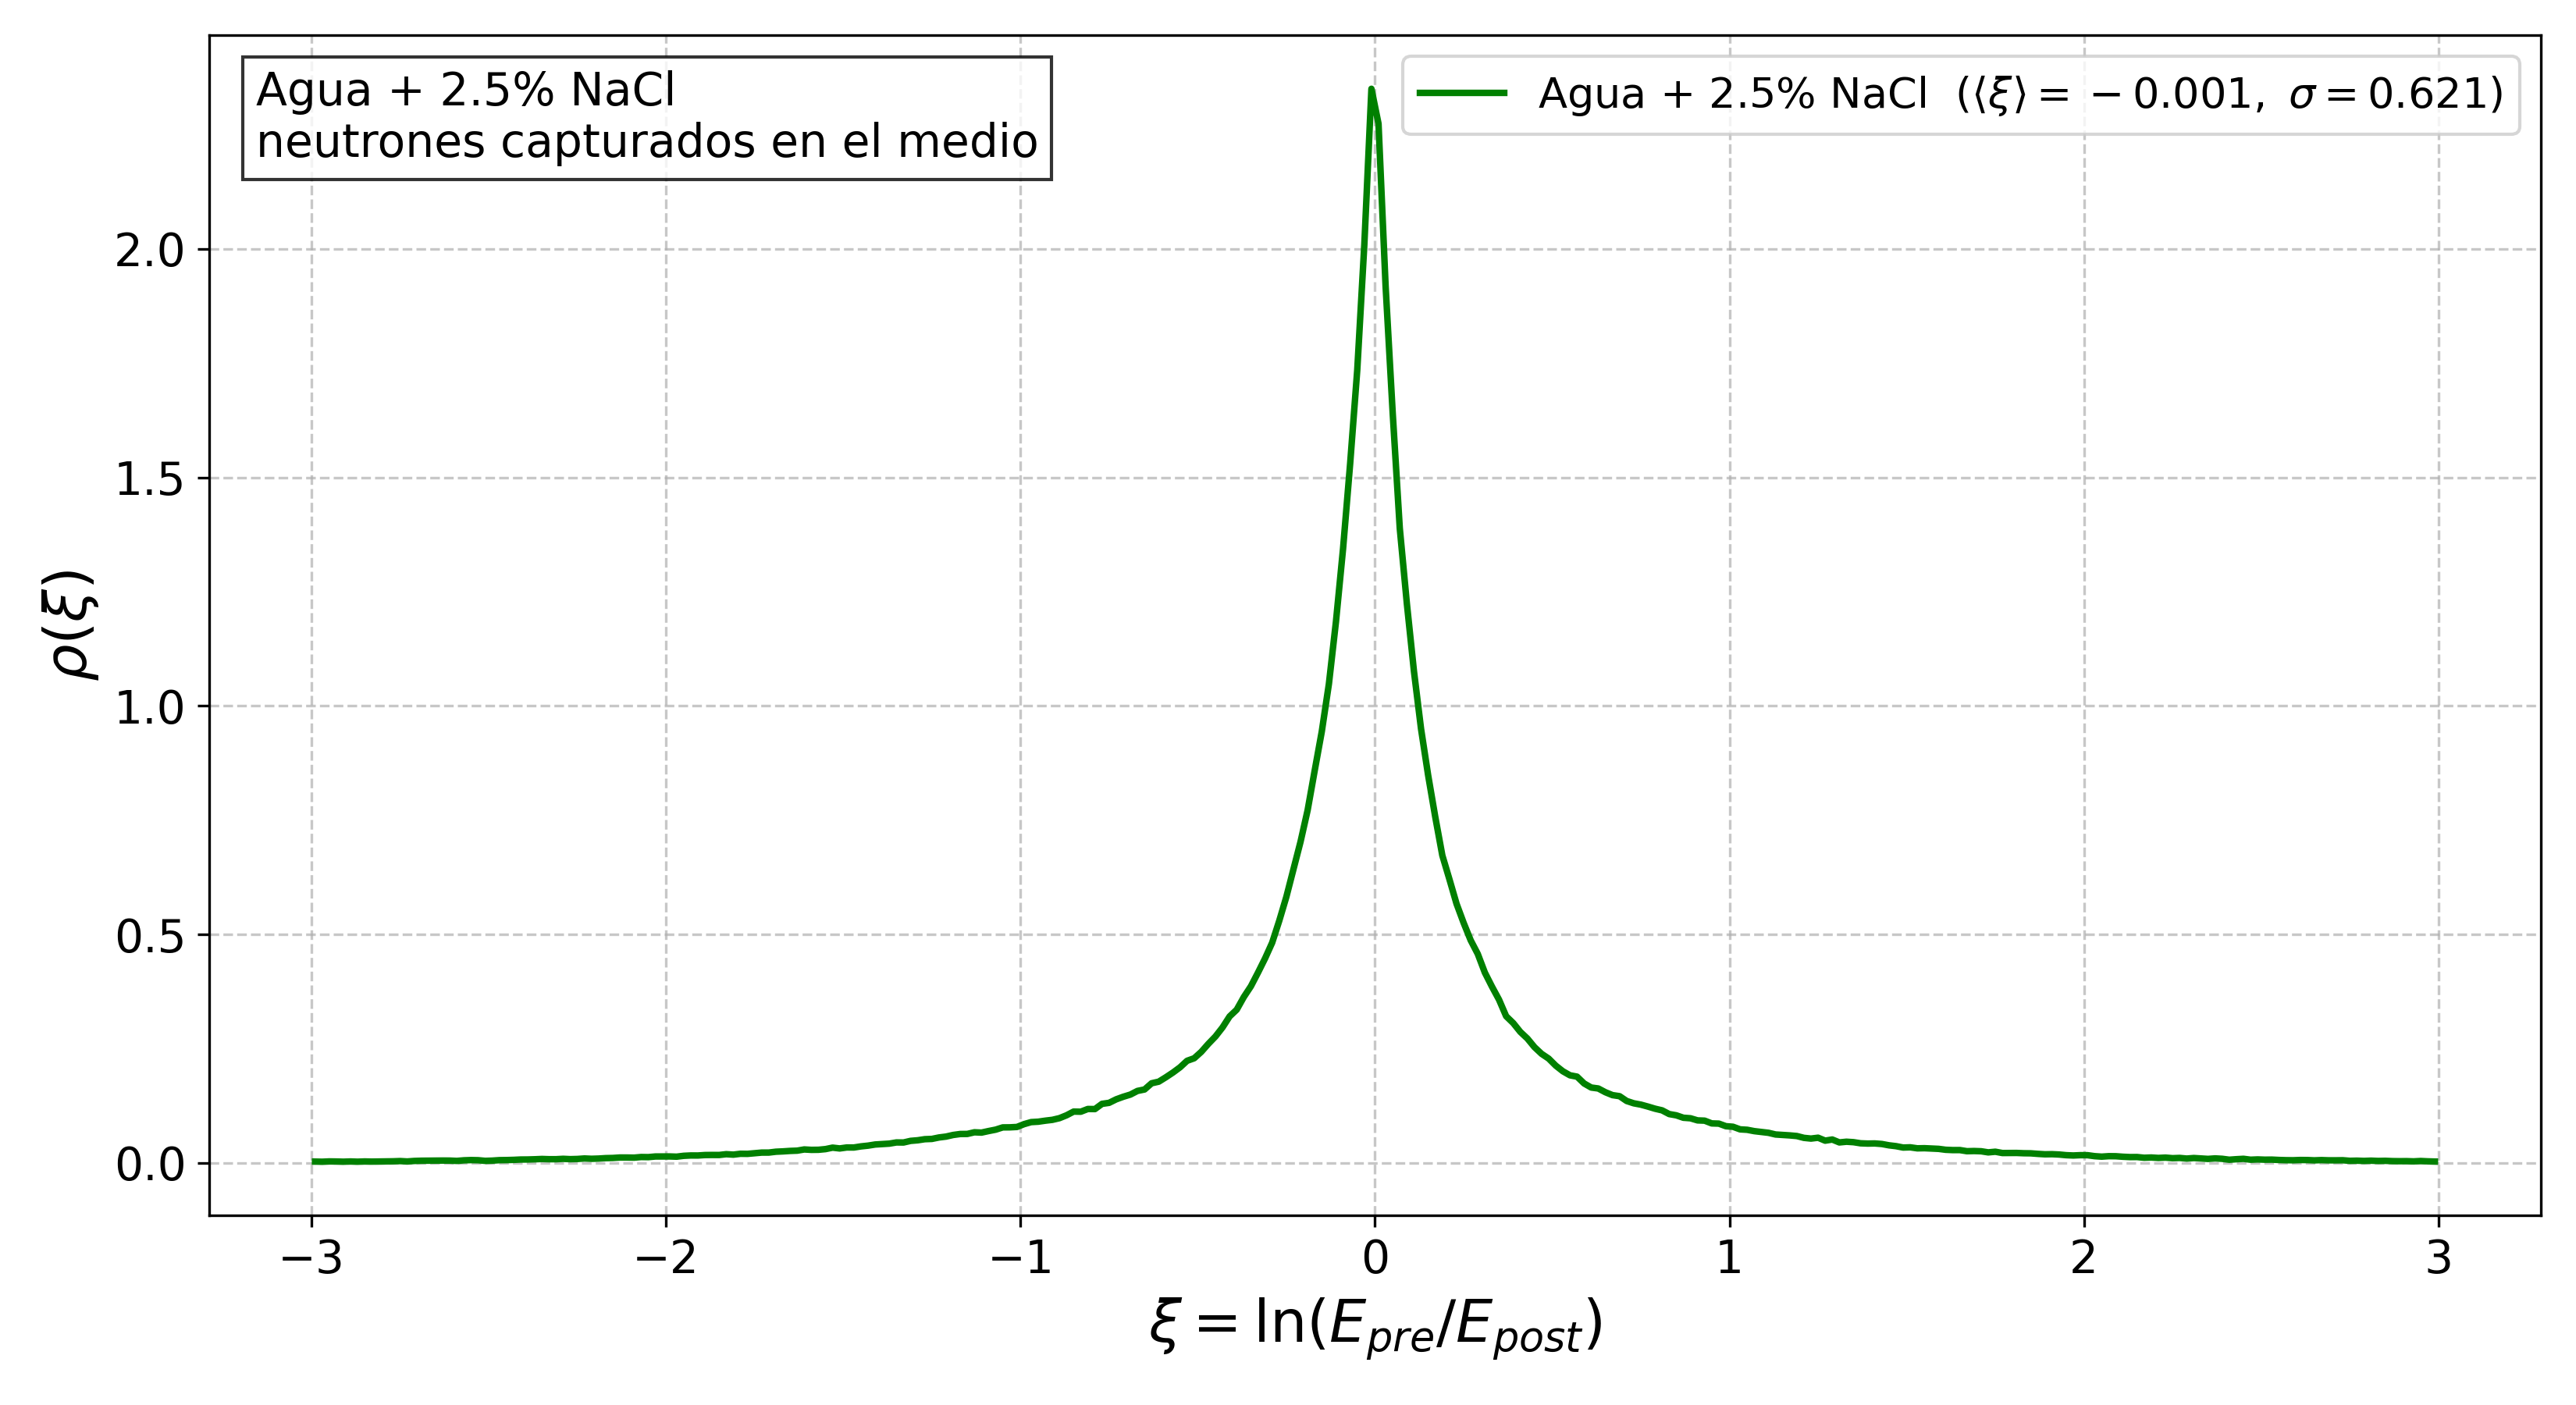
\includegraphics[width=\linewidth]{figuras-analisis-moderacion/nacl25_06a_xi.png}
    \caption{Agua + 2.5\,\% NaCl}
  \end{subfigure}
  \caption{Densidad de probabilidad de $\xi$ por colisión elástica. La forma es prácticamente
  idéntica entre medios -- $\xi$ depende del núcleo con el que colisiona el neutrón (hidrógeno en
  ambos casos, ya que la dispersión elástica sigue dominada por el agua), no de la concentración de
  sal, que afecta sobre todo la probabilidad de \emph{captura} (ver sección~\ref{sec:tiempo}).}
  \label{fig:xi}
\end{figure}

\subsection{Interacciones previas en la estructura: acero, Tyvek y aire}

Antes de alcanzar el medio activo, un neutrón puede dispersarse elásticamente una o varias veces en
el acero de la carcasa, en el Tyvek del revestimiento interno o en el aire remanente dentro del
tanque. Estas colisiones no contribuyen a la señal del detector, pero caracterizan cuánto
``distorsiona'' la estructura mecánica la trayectoria de entrada de los neutrones -- información
relevante para optimizar el diseño (grosor de blindaje, elección de revestimiento) en futuras
versiones del WCD. La figura~\ref{fig:previa} muestra, para agua pura, cuántos neutrones (de los
100\,000 inyectados) dispersan al menos una vez en cada material antes de ingresar al agua, y cuántas
veces lo hacen.

\begin{figure}[H]
  \centering
  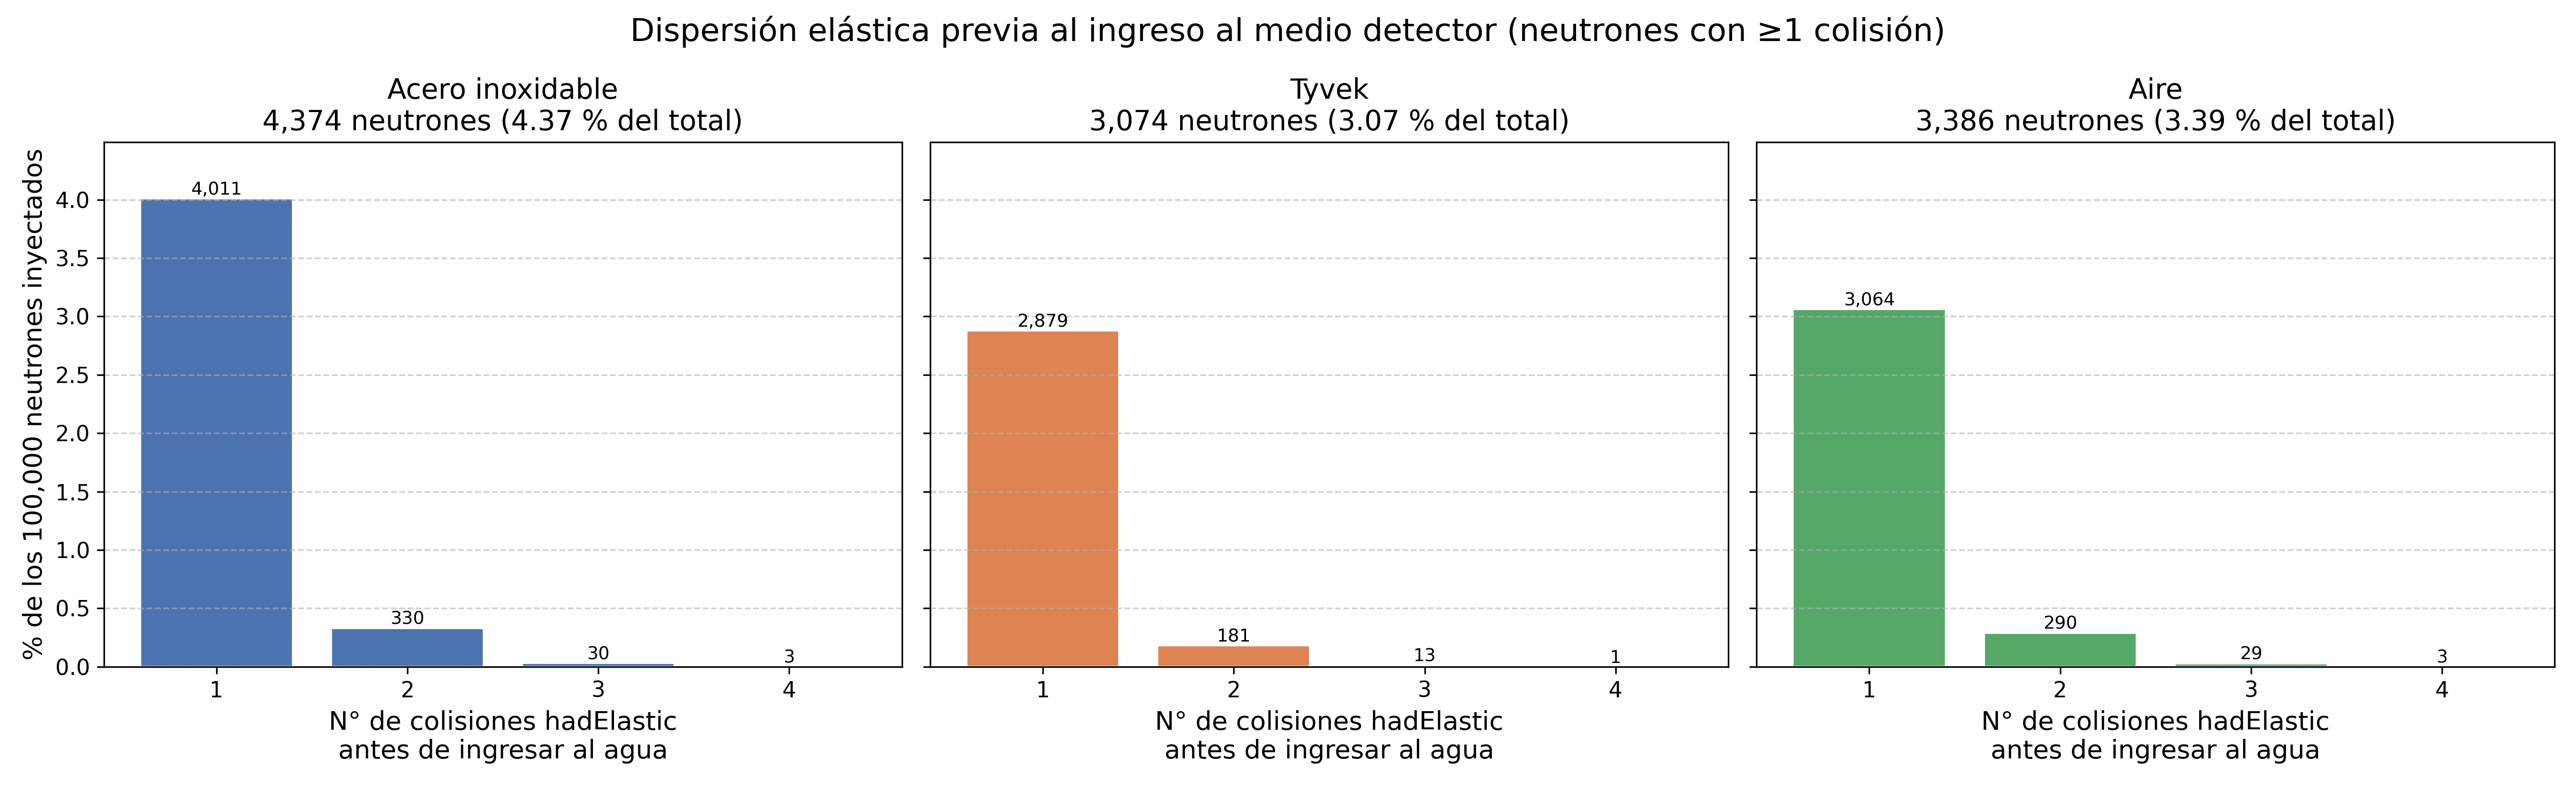
\includegraphics[width=\linewidth]{figuras-analisis-moderacion/agua-pura_07_dispersion_previa.png}
  \caption{Colisiones elásticas previas al ingreso al medio activo, por material (agua pura).}
  \label{fig:previa}
\end{figure}

\subsection{Tiempo hasta la captura, $\Delta t$, y tiempo de decaimiento, $\tau$}
\label{sec:tiempo}

$\Delta t$ es el tiempo transcurrido, para cada neutrón capturado en el medio, entre su primera
dispersión elástica y su captura. Físicamente, la población de neutrones térmicos dentro de un medio
moderador-absorbente decae con el tiempo de forma aproximadamente exponencial,
\begin{equation}
  N(t) \propto e^{-t/\tau},
\end{equation}
donde $\tau$ --el \textbf{tiempo de decaimiento} o \textit{die-away time}-- está directamente ligado
a la sección eficaz macroscópica de absorción del medio, $\Sigma_a$ (a mayor absorción, menor
$\tau$). Esta es, como se explicó en la sección~\ref{sec:contexto}, la misma variable que la
industria petrolera mide con sondas de neutrones pulsados para inferir la salinidad del fluido en un
pozo: el cloro-35 tiene una sección eficaz de captura térmica mucho mayor que el hidrógeno o el
oxígeno, de modo que $\tau$ \emph{disminuye} al aumentar la concentración de NaCl. La
figura~\ref{fig:tau} confirma exactamente ese comportamiento en las dos corridas analizadas: el
histograma de $\Delta t$ en escala logarítmica se ajusta a una recta (es decir, a una exponencial),
excluyendo del ajuste el primer intervalo de tiempo (que concentra capturas casi instantáneas, no
representativas del régimen asintótico de decaimiento).

\begin{figure}[H]
  \centering
  \begin{subfigure}[b]{0.49\linewidth}
    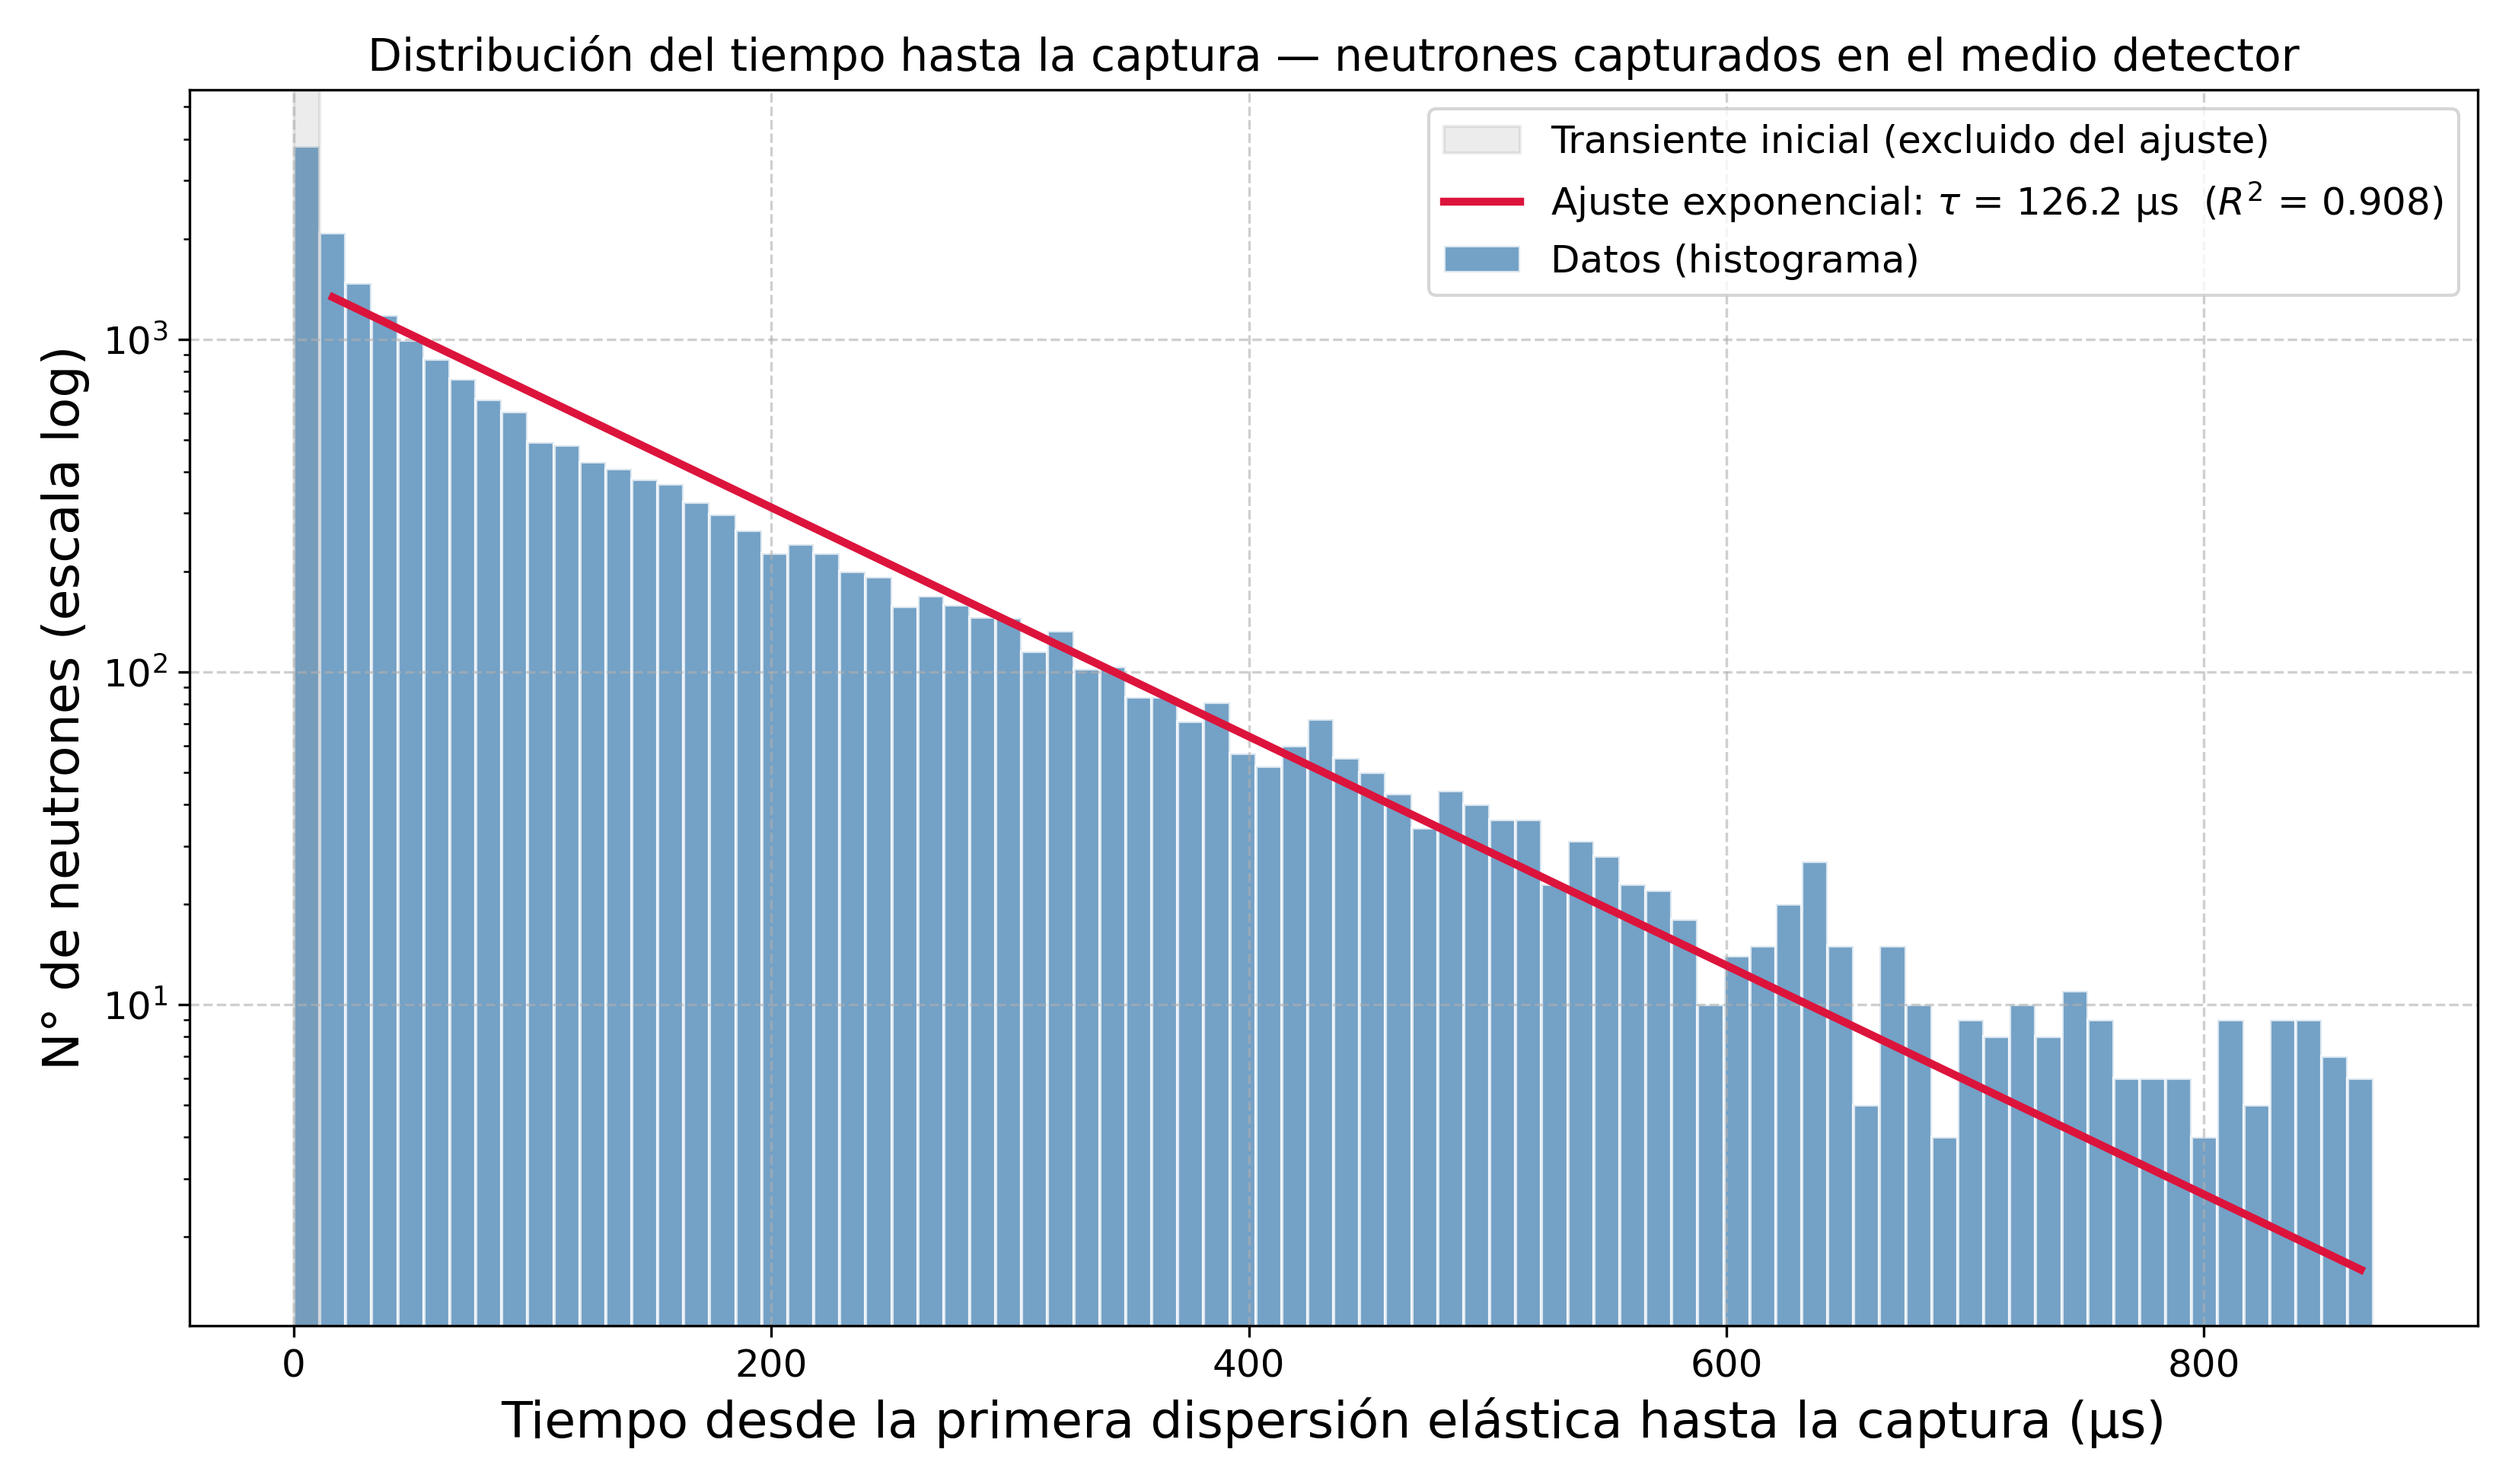
\includegraphics[width=\linewidth]{figuras-analisis-moderacion/agua-pura_08_tiempo.png}
    \caption{Agua pura: $\tau=126.2\,\mu$s}
  \end{subfigure}
  \hfill
  \begin{subfigure}[b]{0.49\linewidth}
    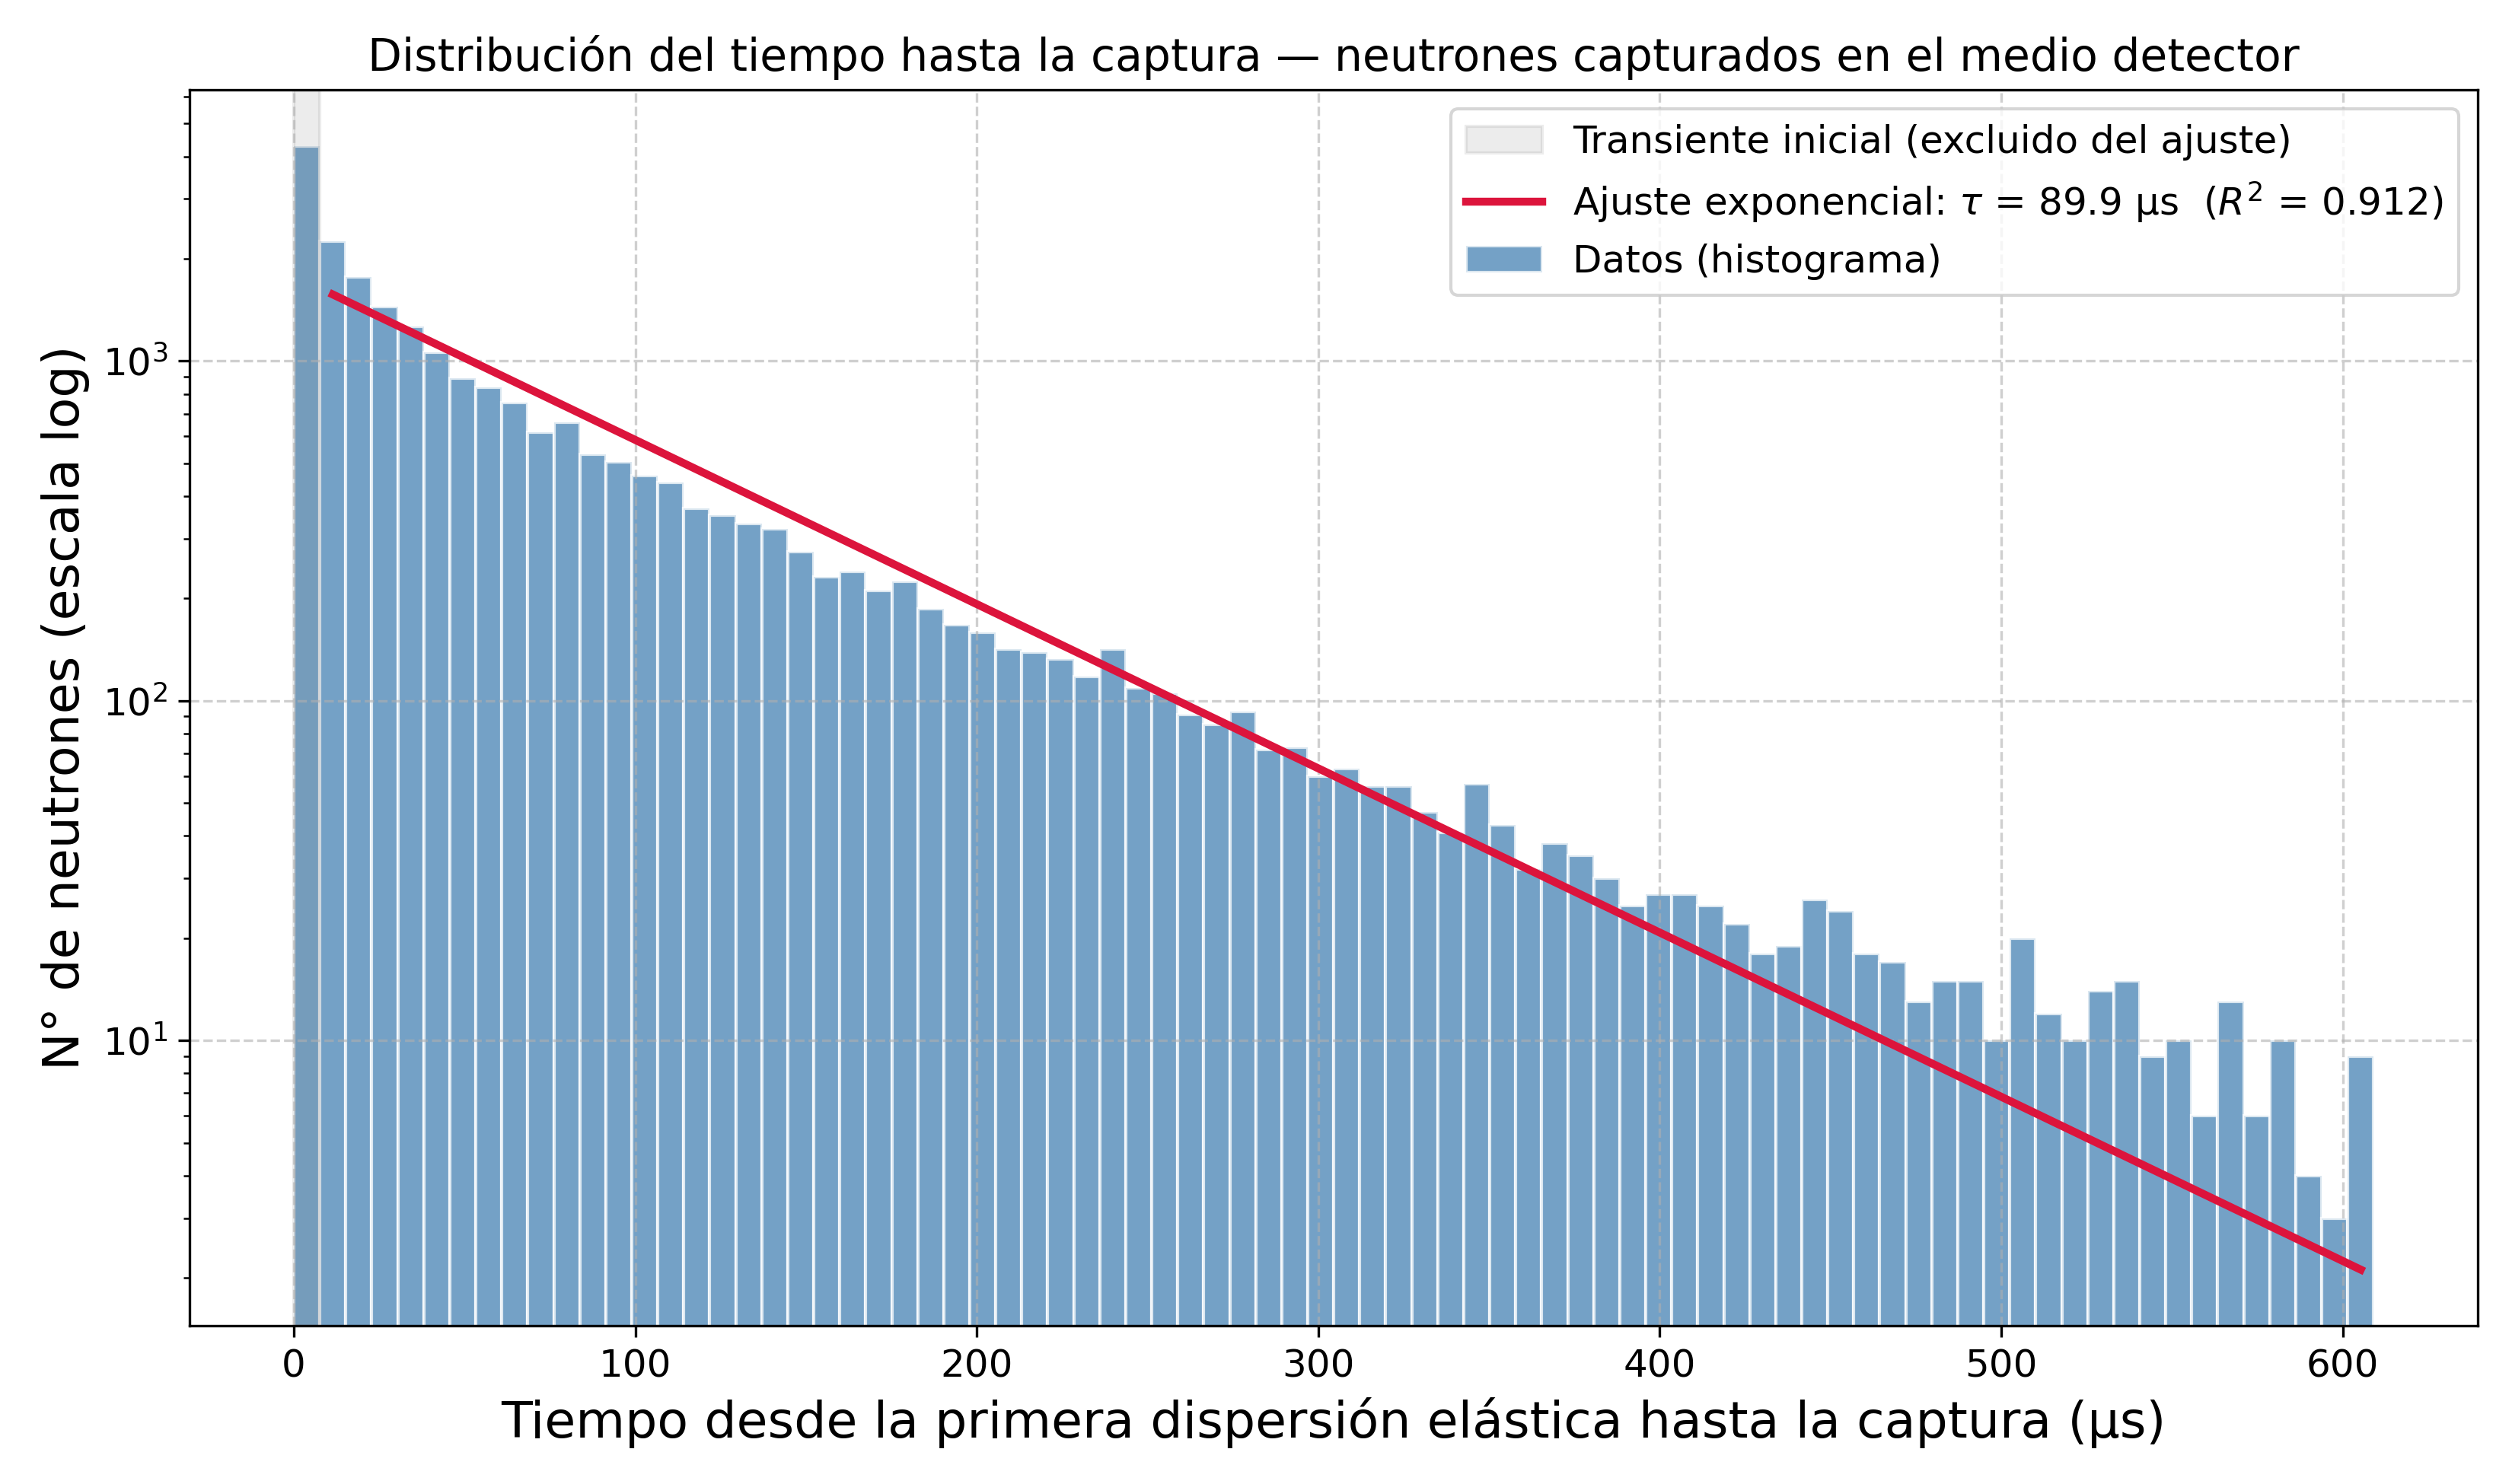
\includegraphics[width=\linewidth]{figuras-analisis-moderacion/nacl25_08_tiempo.png}
    \caption{Agua + 2.5\,\% NaCl: $\tau=89.9\,\mu$s}
  \end{subfigure}
  \caption{Distribución del tiempo hasta la captura y ajuste exponencial. El NaCl reduce el tiempo
  de decaimiento en $\sim$29\,\%, consistente con la mayor sección eficaz de absorción del cloro.}
  \label{fig:tau}
\end{figure}

\section{Resultados comparativos: agua pura frente a agua + 2.5\,\% NaCl}
\label{sec:resultados}

La tabla~\ref{tab:comparativa} resume, para las dos corridas analizadas hasta la fecha de este
informe, todas las variables descritas en la sección~\ref{sec:variables}. Se incluye como ejemplo
del método, no como resultado final de la tesis: falta repetir el mismo análisis para 5\,\% y
10\,\% de NaCl para completar la caracterización de la respuesta del WCD frente a la salinidad.

\begin{table}[H]
\centering
\small
\begin{tabularx}{\linewidth}{X r r}
\toprule
\textbf{Variable} & \textbf{Agua pura} & \textbf{Agua + 2.5\,\% NaCl} \\
\midrule
Neutrones capturados en el medio (de 100\,000) & 19\,623 & 23\,270 \\
Coeficiente de captura en el medio & 19.62\,\% & 23.27\,\% \\
Captura en otro material (estructura) & 3.12\,\% & 3.10\,\% \\
Reflexión & 5.30\,\% & 3.10\,\% \\
Transmisión & 71.95\,\% & 70.53\,\% \\
\midrule
$\langle N\rangle$ (dispersiones antes de captura) & 90.4 & 65.4 \\
Mediana de $N$ & 46 & 34 \\
\midrule
$\langle\xi\rangle$ por colisión & $-0.0011$ & $-0.0013$ \\
$\sigma_\xi$ & 0.622 & 0.621 \\
\midrule
$\langle\Delta t\rangle$ (tiempo medio hasta la captura) & 114.6\,$\mu$s & 82.0\,$\mu$s \\
$\tau$ (ajuste exponencial, die-away) & 126.2\,$\mu$s ($R^2=0.908$) & 89.9\,$\mu$s ($R^2=0.912$) \\
\midrule
Neutrones que dispersan $\geq\!1$ vez en acero antes de ingresar & 4.37\,\% & 4.47\,\% \\
Neutrones que dispersan $\geq\!1$ vez en Tyvek antes de ingresar & 3.07\,\% & 3.27\,\% \\
\bottomrule
\end{tabularx}
\caption{Comparación de las variables de caracterización entre agua pura y agua con 2.5\,\% de NaCl
(100\,000 neutrones primarios, 25\,meV, misma geometría de tanque).}
\label{tab:comparativa}
\end{table}

El patrón es consistente en las tres variables que dependen de la absorción del medio (captura,
$N$ y $\tau$): añadir NaCl aumenta la probabilidad de captura por colisión, de modo que los
neutrones necesitan, en promedio, \emph{menos} colisiones y \emph{menos} tiempo para capturarse.
En cambio, $\xi$ --que depende de la \emph{dispersión} elástica, no de la captura-- es prácticamente
idéntico entre ambos medios, como se explicó en la sección~\ref{sec:xi}. Esta separación entre
``lo que cambia con la sal'' (captura, $N$, $\tau$) y ``lo que no cambia'' ($\xi$) es, en sí misma,
información útil para el diseño de un futuro esquema de inversión humedad/salinidad a partir de
mediciones de campo del WCD.

\section{Relación con la aplicación final del WCD}

Retomando el objetivo planteado en la sección~\ref{sec:contexto}: un WCD desplegado en campo para
CRNS no mide directamente la humedad del suelo, sino una tasa de conteo de neutrones que depende de
\emph{ambas} cosas: cuánta agua hay en el suelo (que modera y remueve neutrones del flujo cósmico
antes de que lleguen al detector) y, en suelos salinos, cuánto cloro hay disuelto en esa agua (que
además absorbe neutrones térmicos con mucha eficiencia). Separar ambos efectos a partir de un único
número (la tasa de conteo) no es posible sin información adicional.

Los resultados de este informe muestran que el propio WCD, gracias a su capacidad de resolver
\emph{tiempo} y no solo conteo, puede en principio aportar esa información adicional: el tiempo de
decaimiento $\tau$ de la señal de captura --si el detector puede resolver temporalmente los pulsos
Cherenkov asociados a cada captura-- es sensible a la salinidad de forma mucho más directa que el
conteo total, exactamente como ocurre en el registro de neutrones pulsados usado en pozos
petroleros. Este es el argumento físico central para justificar por qué vale la pena caracterizar
$\tau$ (y no solo el coeficiente de captura) en cada concentración de NaCl simulada: un WCD que mida
tanto la tasa de captura como el tiempo de decaimiento de esa captura tiene, en principio, dos
observables independientes con los que separar humedad y salinidad --algo que un contador de
neutrones convencional (solo tasa de conteo) no puede hacer por sí solo.

\section{Reproducibilidad}
\label{sec:reprod}

El análisis descrito en este informe se genera con el \textit{notebook}
\codigo{analisis\_moderacion\_captura\_neutrones.ipynb}, que vive junto a los cuatro archivos TSV de
entrada de cada corrida (uno por carpeta de simulación: agua pura, agua + 2.5\,\% NaCl, y así
sucesivamente). El único parámetro que distingue una corrida de otra es el nombre del medio y la
lista de núcleos de captura válidos (\var{NOMBRE\_MEDIO} y \var{NUCLEOS\_MEDIO\_DETECTOR} en la
celda de configuración del \textit{notebook}); todo el resto del código es idéntico entre medios.
Cada ejecución produce, en una subcarpeta \archivo{Salidas/}, los archivos TSV intermedios
numerados (capturas en el medio, ciclo de dispersión-hasta-captura, clasificación
captura/reflexión/transmisión, tiempo hasta la captura, etc.) y las figuras en
\archivo{Salidas/figuras/} (PNG a 300\,dpi y PDF vectorial), que son la fuente de todas las cifras y
figuras citadas en este informe.

\section{Conclusiones}

Este informe documentó el significado físico y el propósito de cada variable calculada por el
análisis de moderación y captura de neutrones del WCD: el coeficiente de captura en el medio
(eficiencia intrínseca del detector), la reflexión y la transmisión (dos formas distintas de pérdida
de sensibilidad), el número de dispersiones elásticas $N$ y la letargía $\xi$ (caracterización
clásica del poder moderador del medio, usada aquí también como verificación del modelo térmico de
la simulación), el tiempo hasta la captura $\Delta t$ y su tiempo de decaimiento $\tau$ (la variable
con la conexión más directa a la salinidad, por analogía con el registro de neutrones pulsados de
la industria petrolera), y las interacciones previas con la estructura del tanque (acero, Tyvek,
aire). La comparación entre agua pura y agua con 2.5\,\% de NaCl confirma que estas variables
responden de forma físicamente coherente al cambio de medio, y deja planteado el camino natural de
continuación: repetir el mismo análisis, ya parametrizado, para 5\,\% y 10\,\% de NaCl, y así
completar la curva $\tau$ (o coeficiente de captura) \textit{vs.} concentración que serviría de
calibración para un futuro WCD de campo.

\end{document}
